\documentclass[11pt,a4paper]{article}
\usepackage[utf8]{inputenc}\usepackage[T1]{fontenc}\usepackage[brazilian]{babel}
\usepackage[margin=2cm]{geometry}\usepackage{graphicx,booktabs,longtable,amsmath,amssymb,hyperref,float,xcolor,fancyhdr,array}
\definecolor{ink}{HTML}{203448}\definecolor{accent}{HTML}{087F8C}
\hypersetup{colorlinks=true,urlcolor=accent,linkcolor=ink,pdftitle={Previsão de traços e reconhecimento de desenhos},pdfauthor={Pedro Martineli}}
\setlength{\parindent}{0pt}\setlength{\parskip}{6pt}\setlength{\headheight}{14pt}
\pagestyle{fancy}\fancyhf{}\fancyhead[L]{\small Projeto 4 — Modelagem temporal de desenhos}\fancyhead[R]{\small Quick, Draw!}\fancyfoot[C]{\thepage}
\begin{document}\begin{center}{\Large\bfseries\color{ink} Previsão de traços e reconhecimento de desenhos com redes neurais}\\[5pt]
Introdução às Redes Neurais Artificiais\\Pedro Martineli (RA: 193474)
\end{center}\textbf{Resumo.} Comparamos duas tarefas sobre 42 mil desenhos do Quick, Draw!. Uma GRU prevê os próximos 5, 15 ou 30 movimentos da caneta. Para reconhecer desenhos parciais, comparamos uma GRU que acompanha a sequência de pontos com uma MLP que recebe a imagem. Com metade do desenho, a acurácia foi de 82,9\% na GRU e 69,8\% na MLP.
\section*{O que fizemos?}
Usamos o Quick, Draw! para estudar duas tarefas. Primeiro, a GRU prevê os próximos movimentos da caneta a partir do trecho observado e da categoria fornecida. Depois, a GRU e a MLP tentam reconhecer a categoria de um desenho parcial.

Cada desenho guarda a categoria, as coordenadas dos pontos, seus tempos e os limites entre traços. Esses registros formam uma série temporal porque a ordem e os intervalos dos movimentos descrevem como o desenho foi feito. Trabalhamos com 42.000 desenhos de 12 categorias, divididos por desenho inteiro em 36.000 para treino, 3.000 para validação e 3.000 para teste. A validação orienta a escolha dos modelos. O desempenho é medido no teste.

O teste usa as mesmas partições dos estudos anteriores do projeto. O recorte contém desenhos reconhecidos pelo próprio jogo.
\begingroup\small\setlength{\tabcolsep}{4pt}\begin{longtable}{lrr}
\caption{As duas tarefas do projeto}\\
\toprule
Tarefa & Entrada & Saída \\
\midrule\endfirsthead
\toprule
Tarefa & Entrada & Saída \\
\midrule\endhead
\bottomrule\endfoot
Previsão t+k & Movimentos e categoria & Próximos pontos da caneta \\
Reconhecimento & Movimentos ou imagem parcial & Probabilidades das 12 categorias \\
\end{longtable}\endgroup
\clearpage
\section*{Como medimos os resultados}
Na previsão, medimos a distância entre os pontos previstos e os pontos registrados. No reconhecimento, contamos quantas categorias as redes acertam.
\subsection*{Previsão — ADE e FDE}
Para cada passo futuro, comparamos o ponto previsto com o ponto registrado no mesmo passo. Calculamos a distância em linha reta, em pixels, a partir das diferenças em X e Y. ADE (Average Displacement Error) é a média dessas distâncias ao longo dos k passos. FDE (Final Displacement Error) usa apenas a distância no último passo. Menor é melhor nas duas métricas.

Exemplo com cinco passos. Se as distâncias são 2, 4, 4, 5 e 10 pixels, o ADE é (2 + 4 + 4 + 5 + 10) / 5 = 5 pixels e o FDE é 10 pixels. Nesse caso, o ponto final ficou mais distante do que a média do trajeto.
\[
d_j=\sqrt{(\widehat{x}_{t+j}-x_{t+j})^2+(\widehat{y}_{t+j}-y_{t+j})^2},\qquad\mathrm{ADE}_k=\frac{1}{k}\sum_{j=1}^{k}d_j,\qquad\mathrm{FDE}_k=d_k.
\]
\subsection*{Reconhecimento — acurácia}
Para cada desenho, usamos como palpite a categoria com maior probabilidade. Se ela coincide com a categoria correta, contamos um acerto. A acurácia é a porcentagem de desenhos acertados. Calculamos essa porcentagem separadamente com 25\%, 50\%, 75\% e 100\% dos eventos disponíveis. As duas redes recebem o mesmo trecho em cada corte.

Exemplo com dez desenhos pela metade. Se o primeiro palpite da rede acerta a categoria em oito deles, a acurácia nesse corte é 8 / 10 = 80\%.
\[
\text{Acurácia (\%)}=100\,\frac{\text{número de desenhos acertados}}{\text{número de desenhos avaliados}}.
\]
\subsection*{De onde vêm os valores do relatório?}
Na tabela de previsão, calculamos ADE e FDE em cada janela elegível de teste e fazemos a média das janelas para aquele horizonte. No gráfico de reconhecimento, contamos os acertos nos 3.000 desenhos de teste em cada corte. Por fim, fazemos a média dos resultados das três inicializações em cada tarefa.
\clearpage
\part{Previsão dos próximos traços (t+k)}
\section{Como continuar um desenho em andamento?}
Imagine que alguém começou o contorno de um peixe. Conhecemos a categoria e vemos por onde a caneta passou. Queremos estimar por onde ela vai passar a seguir, incluindo onde levanta e quanto tempo leva entre os pontos. Por exemplo, com t=32 e k=15, a GRU recebe os eventos 1 a 32 e prevê os eventos 33 a 47. Testamos horizontes de 5, 15 e 30 eventos.

A entrada tem até 64 eventos observados. Cada um contém deslocamentos X/Y, fim de traço (pen-up), intervalo comprimido com logaritmo e posição X/Y relativa ao primeiro ponto. A GRU lê esses movimentos junto com a categoria fornecida. Seu estado final orienta o decoder, que escolhe e ajusta uma entre 64 trajetórias-base da categoria, aprendidas no treino.
\subsection{Ajuste dos hiperparâmetros da previsão}
Cruzamos duas larguras da GRU com duas taxas iniciais de aprendizagem. Cada treino usou AdamW por 20 épocas. Avaliamos os quatro candidatos com a inicialização 42 e repetimos os dois melhores com a 43. O escore de validação considera distância em pixels, encerramentos antes do horizonte e erros de pen-up. Para cada finalista, também testamos limiares de pen-up de 0,2, 0,35 e 0,5 e escolhemos o menor escore médio.

A configuração selecionada tem 192 unidades ocultas, taxa de 0,001 e limiar de 0,2. A inicialização 44 entra na média final do teste, depois da seleção.
\begingroup\small\setlength{\tabcolsep}{4pt}\begin{longtable}{lrrr}
\caption{Busca da GRU na validação. Menor escore é melhor. A média é calculada para os finalistas.}\\
\toprule
Unidades & Taxa inicial & Escore 42 & Média 42 e 43 \\
\midrule\endfirsthead
\toprule
Unidades & Taxa inicial & Escore 42 & Média 42 e 43 \\
\midrule\endhead
\bottomrule\endfoot
128 & 0,0010 & 0,3963 & 0,3937 \\
128 & 0,0005 & 0,4204 & — \\
192 & 0,0010 & 0,3802 & 0,3800 \\
192 & 0,0005 & 0,4055 & — \\
\end{longtable}\endgroup
\clearpage
\section{Aprendizagem e erro de previsão}
Na tabela, o ADE e o FDE aumentam conforme a GRU prevê mais eventos. Os valores são médias de três inicializações e incluem todas as janelas elegíveis do teste para cada horizonte.
\begingroup\small\setlength{\tabcolsep}{4pt}\begin{longtable}{lrr}
\caption{Resultados da GRU no teste}\\
\toprule
Horizonte k & ADE (pixels) & FDE (pixels) \\
\midrule\endfirsthead
\toprule
Horizonte k & ADE (pixels) & FDE (pixels) \\
\midrule\endhead
\bottomrule\endfoot
5 & 44,7 & 71,3 \\
15 & 94,8 & 149,2 \\
30 & 138,6 & 196,5 \\
\end{longtable}\endgroup
\begin{figure}[H]\centering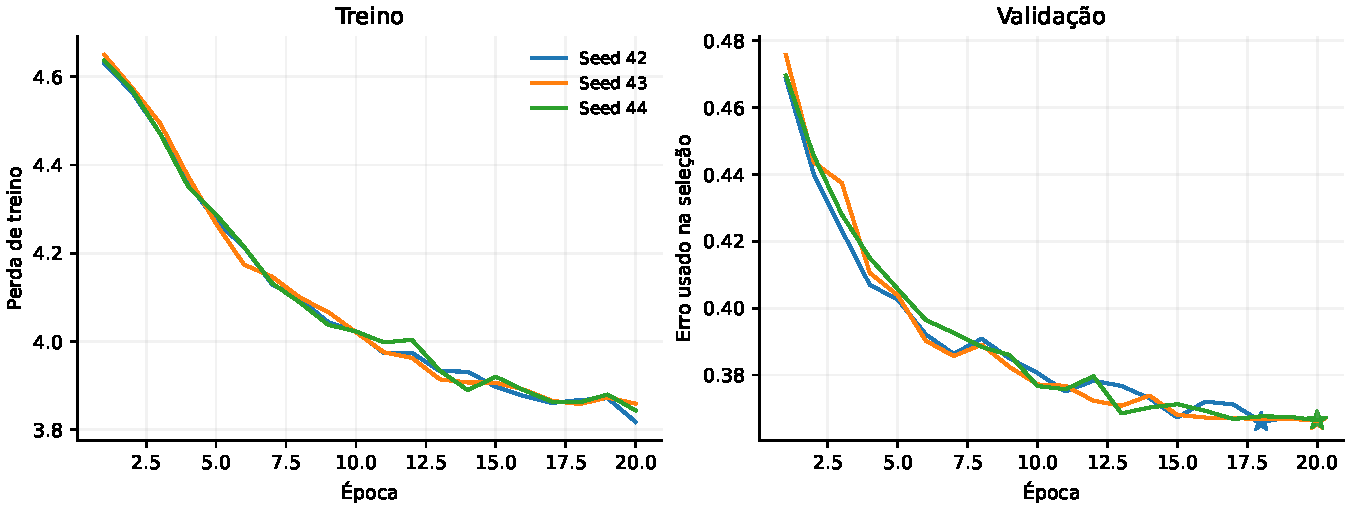
\includegraphics[width=\linewidth,height=.57\textheight,keepaspectratio]{../figures/forecast_gru_learning.pdf}\caption{As estrelas marcam as épocas escolhidas na validação para cada inicialização.}\end{figure}
\clearpage
\subsection*{Cinco continuações dos exemplos de validação}
Os exemplos vêm da validação. Selecionamos trechos com baixo erro de posição e uma continuação visualmente coerente.
\begin{figure}[H]\centering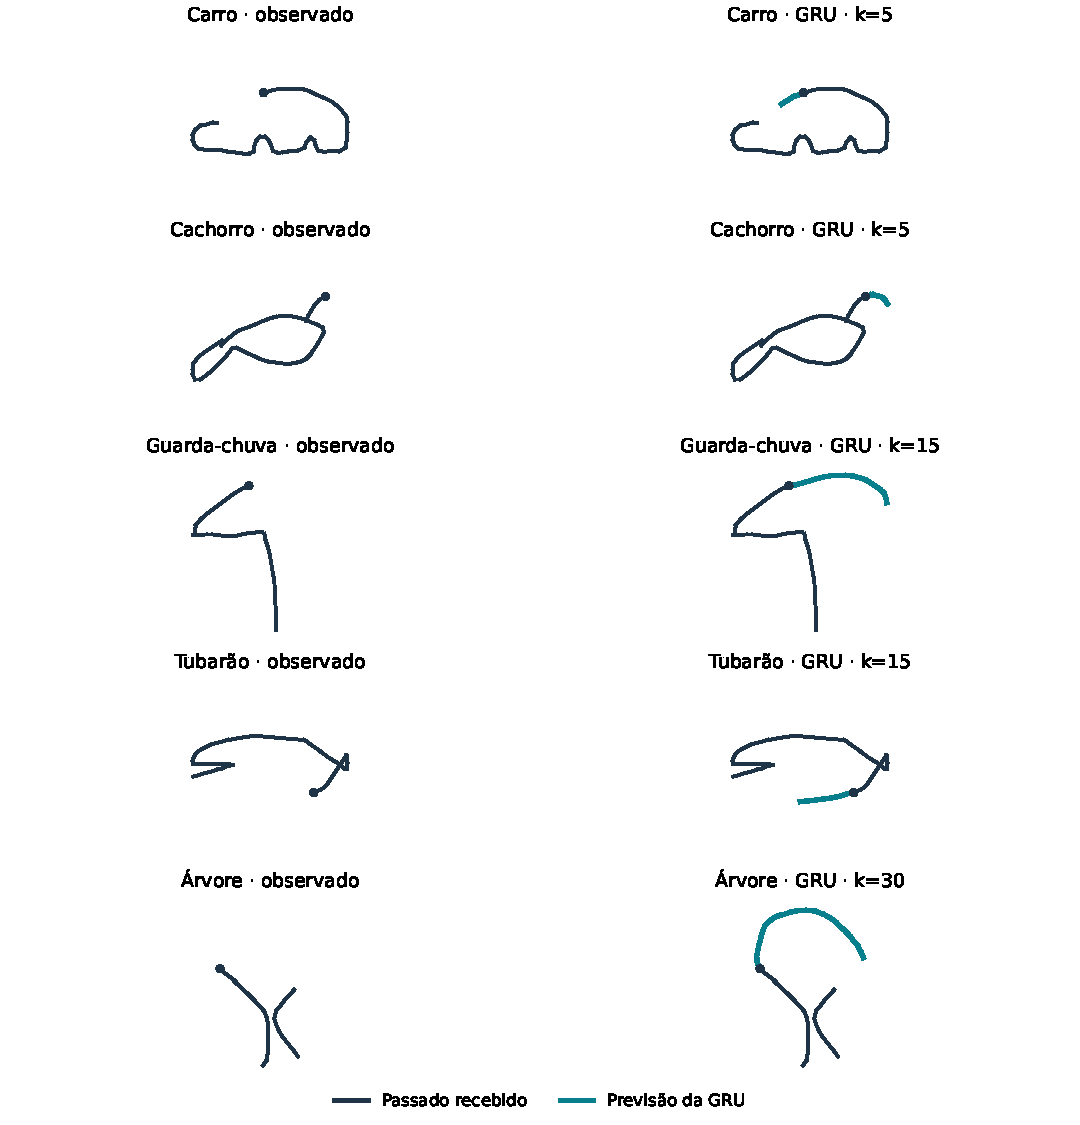
\includegraphics[width=\linewidth,height=.75\textheight,keepaspectratio]{../figures/forecast_apresentacao_casos.pdf}\caption{À esquerda, a entrada. À direita, essa mesma entrada com os pontos previstos pela GRU em verde-azulado.}\end{figure}
\clearpage
\subsection*{Exemplo em detalhe · peixe, k=30}
Categoria fornecida: Peixe. A GRU observa 16 eventos e prevê os próximos 30. ADE de 17,49 px e FDE de 13,37 px. Validação, ID 4765551467429888, seed 42.
\begin{figure}[H]\centering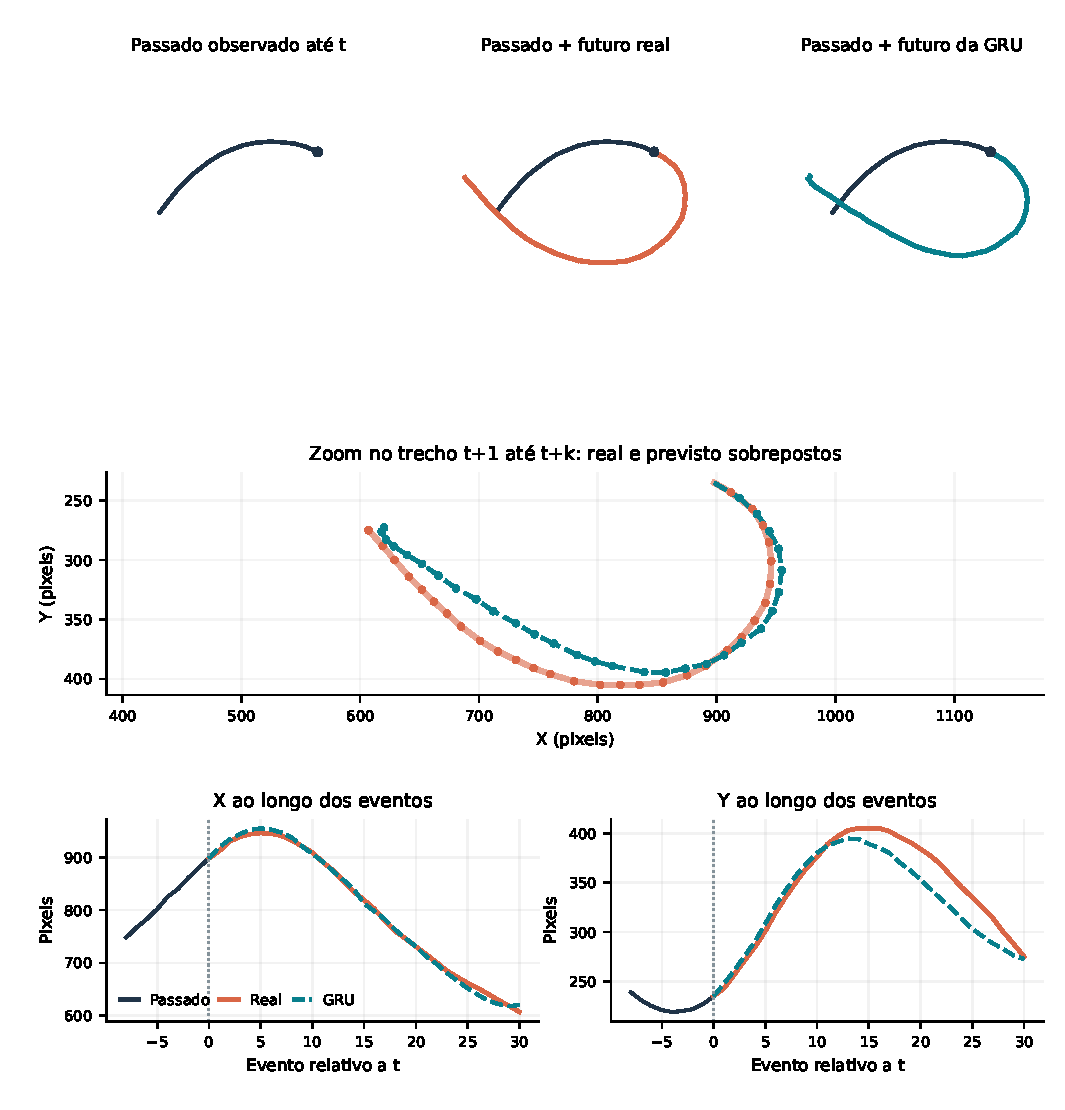
\includegraphics[width=\linewidth,height=.75\textheight,keepaspectratio]{../figures/forecast_success_06_4765551467429888_k30.pdf}\caption{A linha escura mostra os 16 eventos observados. A linha verde-azulada mostra a continuação da GRU para os 30 eventos seguintes. As curvas detalham as coordenadas X e Y.}\end{figure}
\clearpage
\clearpage
\part{Reconhecimento da categoria do desenho}
\section{Quando já dá para reconhecer o desenho?}
Um arco isolado pode ser o começo de um peixe, de uma flor ou de um guarda-chuva. Queremos saber em que momento os traços já permitem reconhecer a categoria. Mostramos às duas redes o mesmo desenho em quatro estágios e pedimos um palpite entre 12 classes.

A GRU recebe os movimentos em sequência, com tempos e fins de traço. A MLP vê a imagem dos pontos já desenhados, em 32 $\times$ 32 pixels achatados em um vetor. Cada rede devolve 12 probabilidades. Comparamos a categoria de maior probabilidade com a categoria correta e observamos como a acurácia muda à medida que chegam novos pontos.
\subsection{Ajuste dos hiperparâmetros do reconhecimento}
Em cada rede, cruzamos duas larguras com duas taxas iniciais e treinamos cada configuração por 32 épocas. Testamos as quatro combinações com a inicialização 42 e repetimos as duas melhores com a 43. O critério foi a menor perda média de validação nos quatro cortes de 25\%, 50\%, 75\% e 100\%. Essa perda, chamada de entropia cruzada, aumenta quando a rede atribui pouca probabilidade à categoria correta.

A GRU escolhida tem 192 unidades e taxa de 0,003. A MLP escolhida tem 256 e 128 unidades ocultas e taxa de 0,001. As duas taxas finalistas da MLP ficaram muito próximas. A inicialização 44 entra na média do teste.
\begingroup\small\setlength{\tabcolsep}{4pt}\begin{longtable}{lrrrr}
\caption{Busca da GRU e da MLP na validação. Menor perda é melhor. A média é calculada para os finalistas.}\\
\toprule
Rede & Largura & Taxa inicial & Perda 42 & Média 42 e 43 \\
\midrule\endfirsthead
\toprule
Rede & Largura & Taxa inicial & Perda 42 & Média 42 e 43 \\
\midrule\endhead
\bottomrule\endfoot
GRU & 128 & 0,003 & 0,57989 & 0,57835 \\
GRU & 128 & 0,001 & 0,99582 & — \\
GRU & 192 & 0,003 & 0,54501 & 0,53929 \\
GRU & 192 & 0,001 & 0,78148 & — \\
MLP de imagem & 128 & 0,003 & 0,92273 & — \\
MLP de imagem & 128 & 0,001 & 0,94818 & — \\
MLP de imagem & 256 & 0,003 & 0,84914 & 0,84845 \\
MLP de imagem & 256 & 0,001 & 0,85127 & 0,84841 \\
\end{longtable}\endgroup
\clearpage
\section{Como as redes aprenderam}
Para cada configuração escolhida, usamos os pesos da época com menor perda de validação. As curvas mostram como a perda evoluiu ao longo das épocas nas três inicializações.
\begin{figure}[H]\centering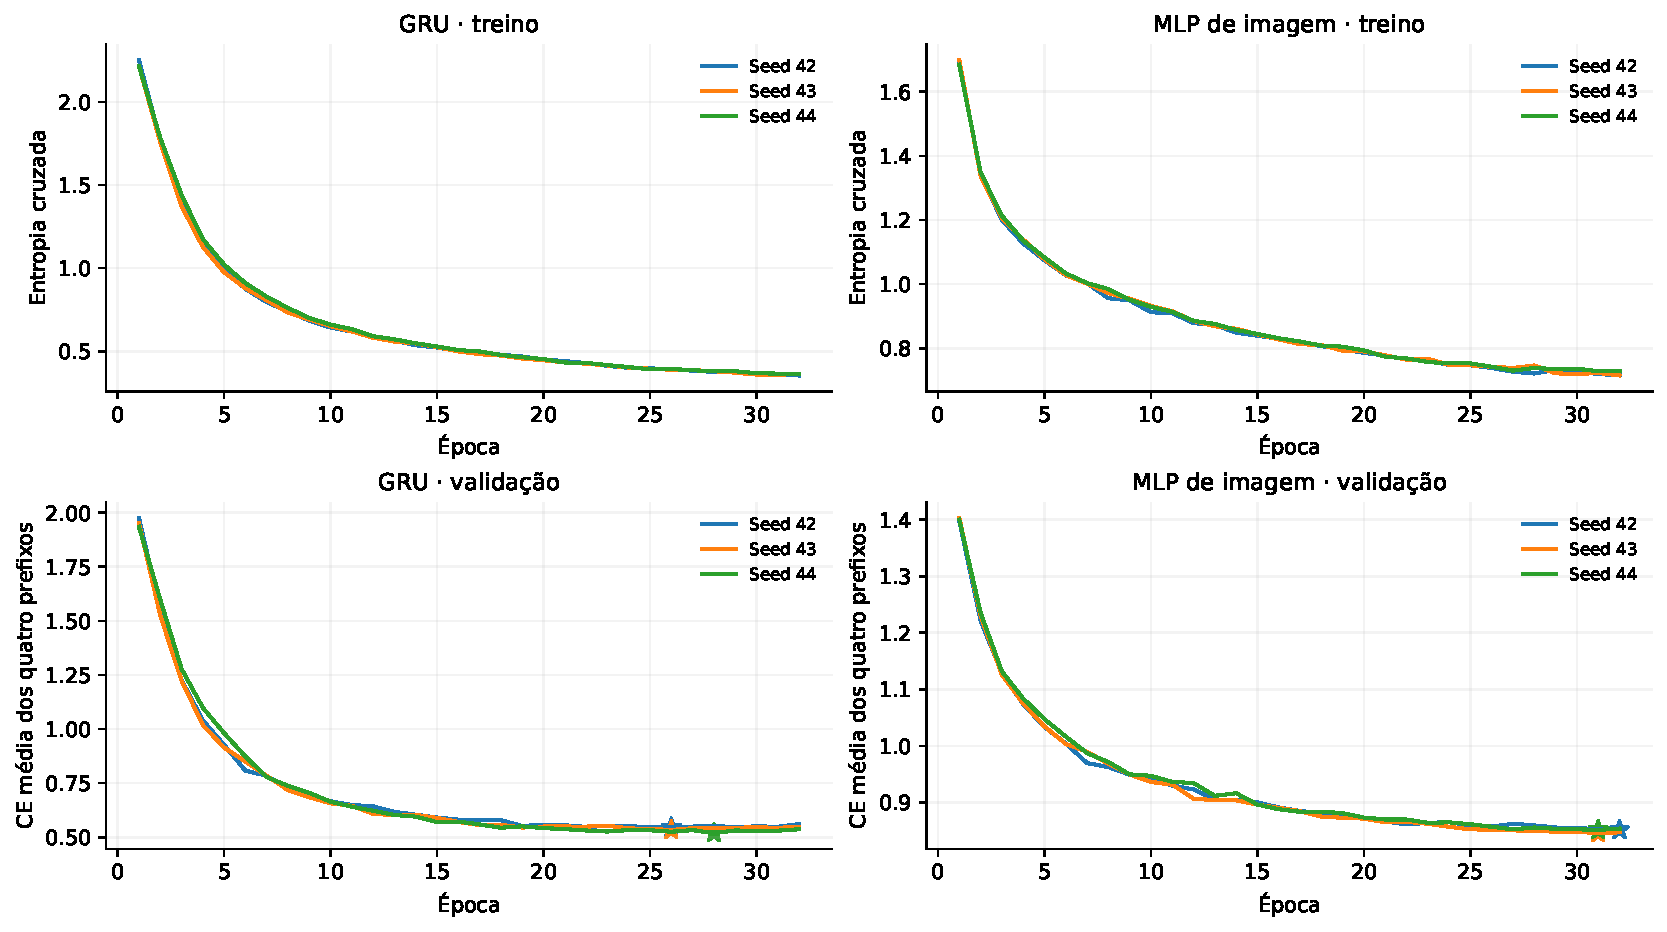
\includegraphics[width=\linewidth,height=.57\textheight,keepaspectratio]{../figures/02_aprendizagem.pdf}\caption{Curvas de treino e validação das duas redes. As estrelas marcam as épocas escolhidas com base na validação.}\end{figure}
\clearpage
\section{Acurácia conforme o desenho aparece}
Com metade do desenho, a GRU acertou 82,9\% e a MLP acertou 69,8\%. Com o desenho completo, os resultados foram 93,0\% e 83,7\%, respectivamente. Nos quatro cortes avaliados, a GRU teve maior acurácia. As redes usam arquiteturas e representações diferentes, então a comparação mede o efeito dessas escolhas em conjunto.

As próximas páginas mostram quatro desenhos de validação com resultados diferentes. No peixe desenhado livremente no site, a GRU atribuiu 97,5\% a Peixe e o palpite principal da MLP foi Cachorro (33,9\%). O peixe mostrado a seguir é outro desenho, de validação, com uma confusão semelhante.
\begin{figure}[H]\centering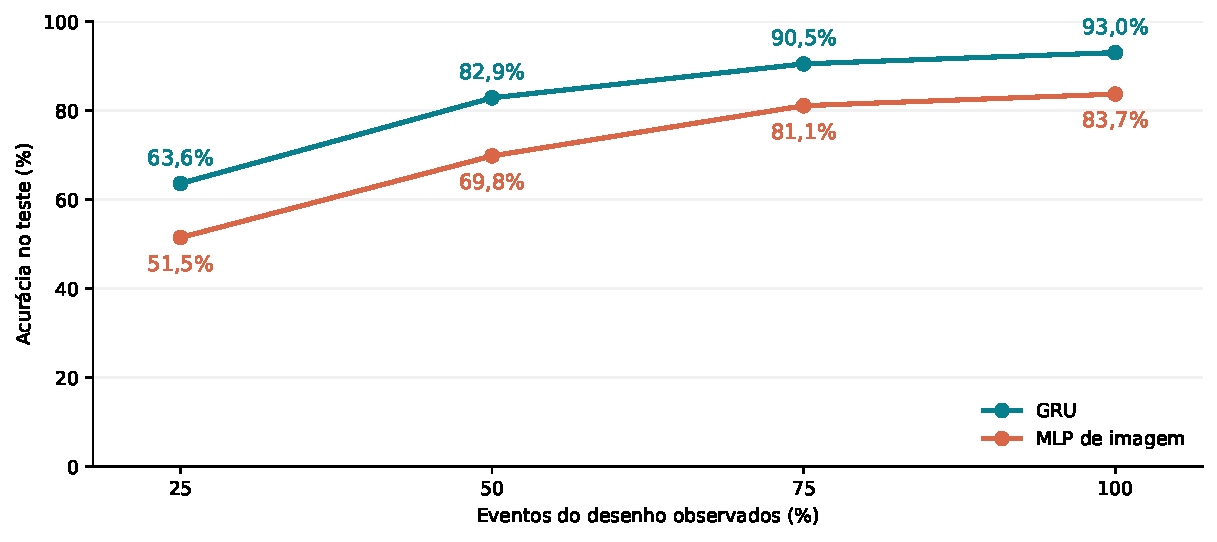
\includegraphics[width=\linewidth,height=.57\textheight,keepaspectratio]{../figures/reconhecimento_acuracia_apresentacao.pdf}\caption{Acurácia depois de observar 25\%, 50\%, 75\% e 100\% dos eventos.}\end{figure}
\clearpage
\subsection*{Peixe · a GRU encontra a categoria}
Nos últimos eventos, a GRU reconhece o peixe e a MLP dá sua maior probabilidade a Cachorro.
\begin{figure}[H]\centering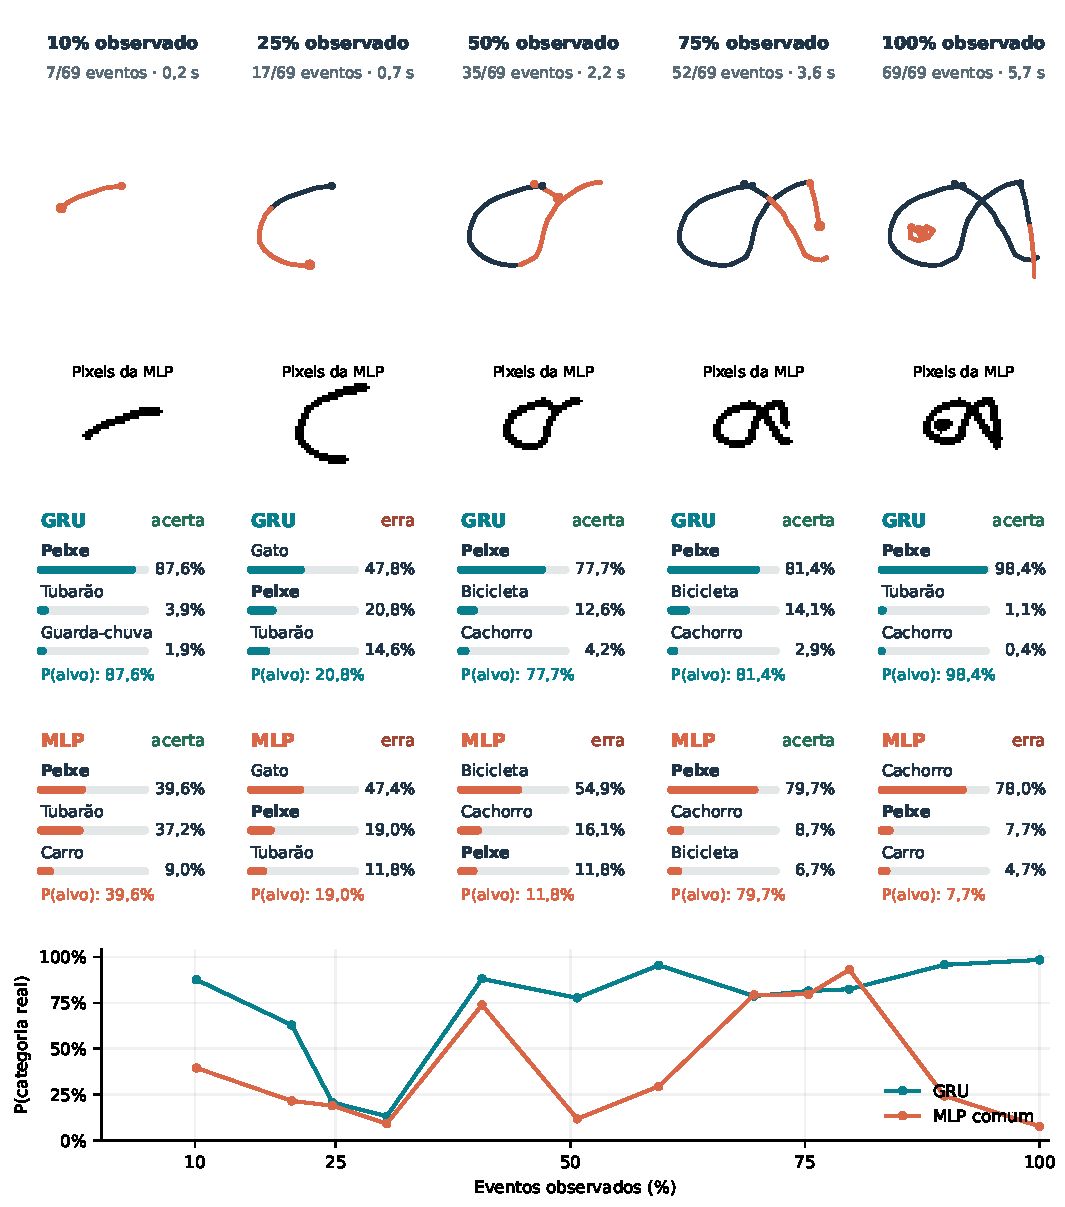
\includegraphics[width=\linewidth,height=.75\textheight,keepaspectratio]{../figures/gallery_01_5421316351983616.pdf}\caption{As colunas revelam 10\%, 25\%, 50\%, 75\% e 100\% dos eventos. A imagem em preto e branco é a entrada da MLP. As barras mostram os três palpites de cada rede. A curva mostra a probabilidade da categoria correta.}\end{figure}
\clearpage
\subsection*{Flor · a GRU acerta com metade do desenho}
Os palpites dividem-se enquanto o contorno ainda está incompleto.
\begin{figure}[H]\centering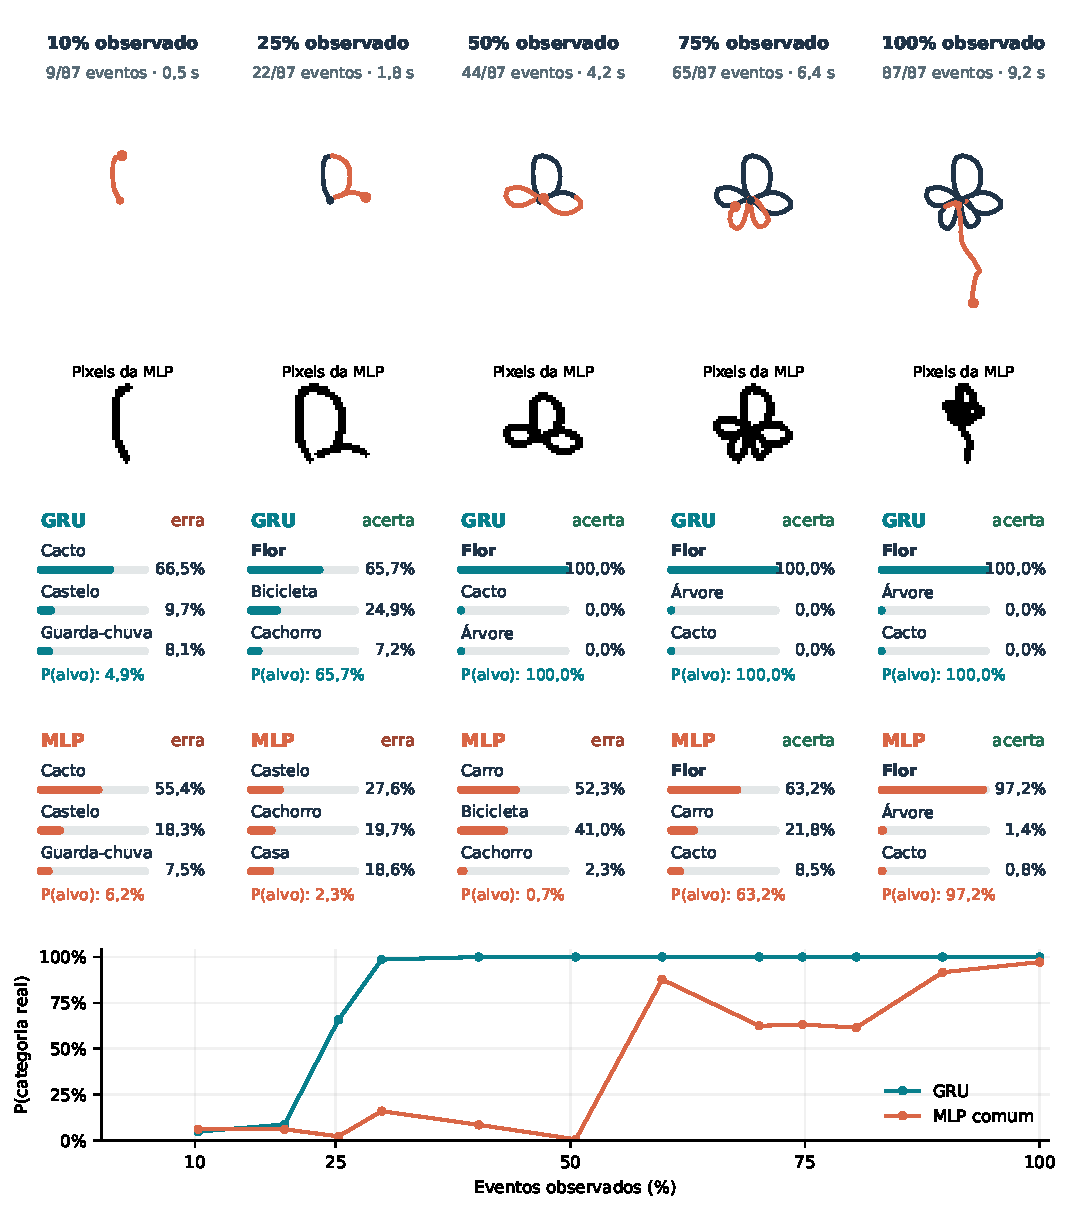
\includegraphics[width=\linewidth,height=.75\textheight,keepaspectratio]{../figures/gallery_04_6342047466258432.pdf}\caption{As colunas revelam 10\%, 25\%, 50\%, 75\% e 100\% dos eventos. A imagem em preto e branco é a entrada da MLP. As barras mostram os três palpites de cada rede. A curva mostra a probabilidade da categoria correta.}\end{figure}
\clearpage
\subsection*{Guarda-chuva · as duas redes reconhecem}
Os novos traços tornam a forma mais clara para as duas redes.
\begin{figure}[H]\centering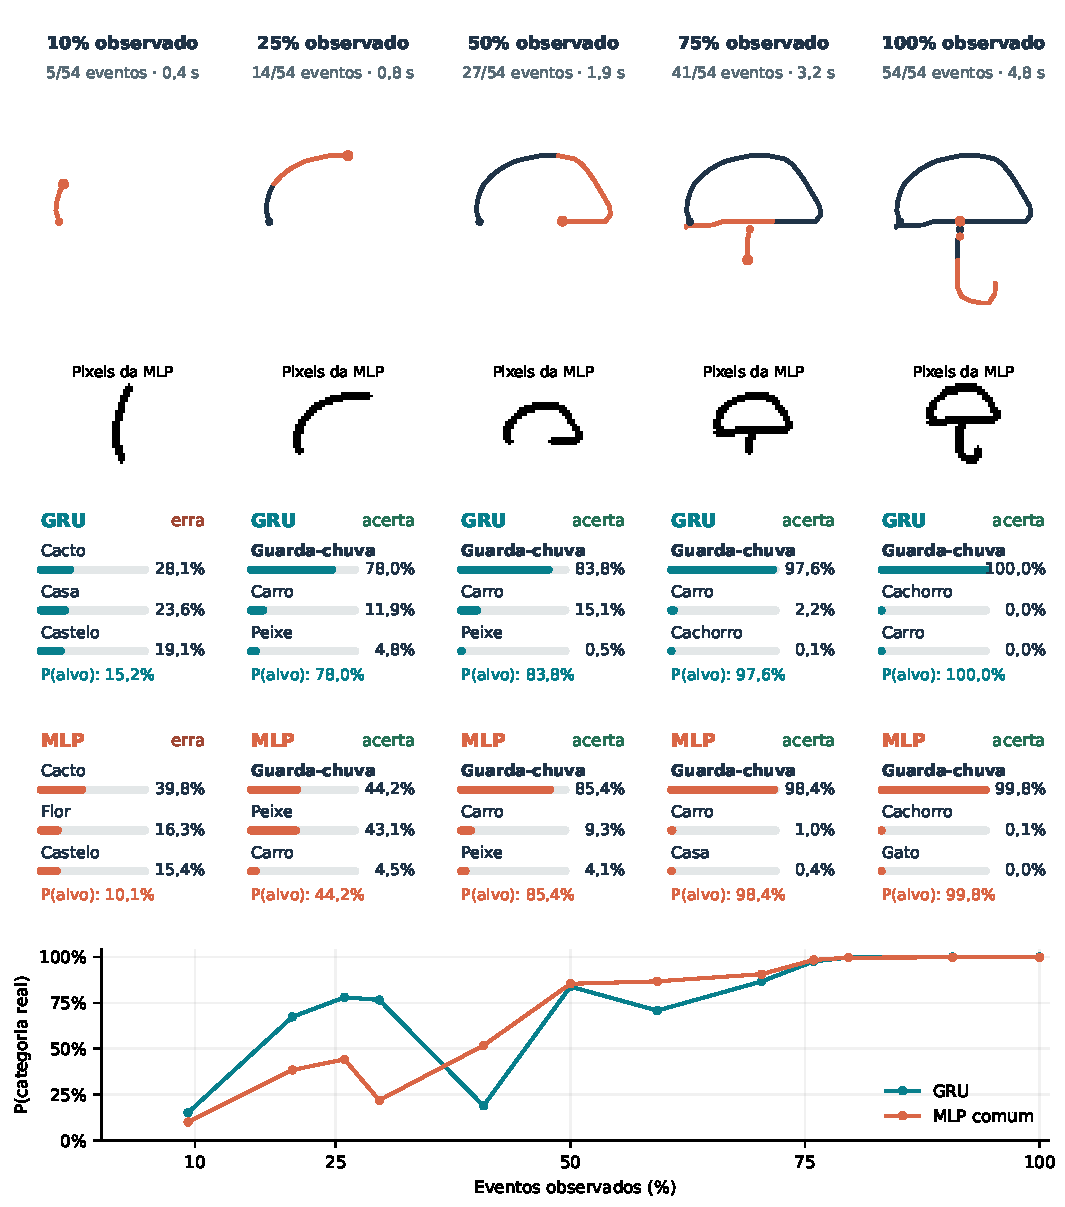
\includegraphics[width=\linewidth,height=.75\textheight,keepaspectratio]{../figures/gallery_07_6511453274112000.pdf}\caption{As colunas revelam 10\%, 25\%, 50\%, 75\% e 100\% dos eventos. A imagem em preto e branco é a entrada da MLP. As barras mostram os três palpites de cada rede. A curva mostra a probabilidade da categoria correta.}\end{figure}
\clearpage
\subsection*{Carro · a MLP reconhece mais cedo neste caso}
Neste desenho, com 50\% dos pontos, a MLP acerta e a GRU ainda erra.
\begin{figure}[H]\centering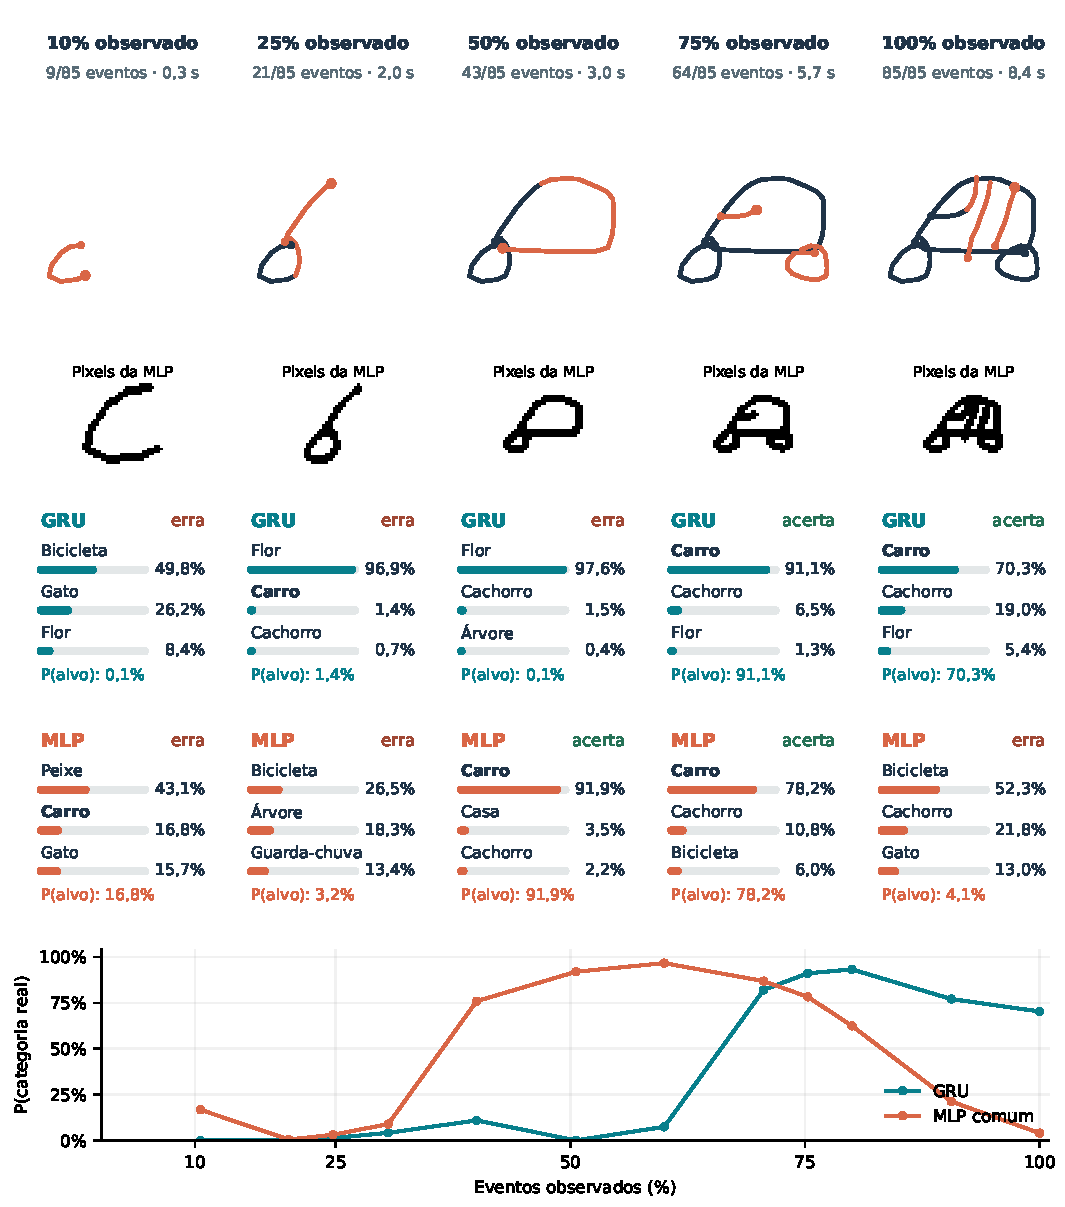
\includegraphics[width=\linewidth,height=.75\textheight,keepaspectratio]{../figures/gallery_12_6141759400706048.pdf}\caption{As colunas revelam 10\%, 25\%, 50\%, 75\% e 100\% dos eventos. A imagem em preto e branco é a entrada da MLP. As barras mostram os três palpites de cada rede. A curva mostra a probabilidade da categoria correta.}\end{figure}
\clearpage
\section{O que os resultados mostram}
A GRU consegue continuar trechos curtos da caneta em exemplos como os da galeria. No teste, a previsão fica mais difícil conforme o horizonte cresce. No reconhecimento, as duas redes acertam mais quando recebem uma parte maior do desenho. A GRU obteve a maior acurácia média nos quatro cortes, e a galeria também inclui um exemplo em que a MLP acerta mais cedo.
\section*{Referências}\begin{enumerate}
\item \href{https://github.com/googlecreativelab/quickdraw-dataset}{Google Creative Lab — Quick, Draw! Dataset e licença CC BY 4.0}
\item \href{https://arxiv.org/abs/1406.1078}{Cho et al. (2014) — artigo que apresenta a GRU}
\item \href{https://martinelipedro.github.io/projeto4-irn/forecast/}{Laboratório de previsão da GRU}
\item \href{https://martinelipedro.github.io/projeto4-irn/}{Laboratório de reconhecimento da GRU e da MLP}
\item \href{https://github.com/martinelipedro/projeto4-irn}{Código, galeria completa e resultados do projeto}
\end{enumerate}\small Dados: Google Quick, Draw!, CC BY 4.0. Código e redação elaborados com auxílio de IA; resultados acompanhados de artefatos e verificações numéricas.\end{document}